\documentclass[12pt,a4paper]{article}

\usepackage[utf8]{inputenc}
\usepackage[a4paper,total={150mm,240mm}]{geometry}
\usepackage[american]{babel}

\usepackage{float}
\usepackage{babel}
\usepackage{amsmath}
\usepackage{tikz}
\usepackage{graphicx}
\usepackage{amssymb}
\usepackage{wrapfig}
\usepackage{todonotes}


\usepackage{listings}
\definecolor{listingbg}{gray}{0.95}
\lstset{
  language=C++,
  basicstyle=\ttfamily\small,
  frame=single,
  backgroundcolor=\color{listingbg},
  breaklines=true,
  postbreak=\raisebox{0ex}[0ex][0ex]{\ensuremath{\color{red}\hookrightarrow\space}}
  }


% Exercise stylesheet
\usepackage{exercise}

\title{\textbf{Exercises for Tutorial03}}
\subtitle{Instationary Parabolic Equations}
\exerciselabel{Exercise}




\begin{document}

\exerciseheader

\begin{Exercise}{Getting to Know the Code}
  \lstset{language=bash}
  The code of \lstinline!tutorial03! solves the problem
  \begin{align}
    \partial_t u-\Delta u+q(u) &= f && \text{in }\Omega\times\Sigma =
    (0,1)^d \times (t_0, T], \\
    u(x,t) & =g(x,t) && \text{on }\Gamma_D\subseteq\partial\Omega, \\
    -\nabla u(x,t) \cdot \vec{n} &= j(x,t) &&
    \text{on }\Gamma_N=\partial\Omega\setminus\Gamma_D, \\
    u(x,t_0)&=u_0(x) && \text{at } t=t_0
  \end{align}
  with the following choices applied:
  \begin{align}
    \label{ch1:first}
    q(u) &= \eta u^2 \\
    f &= 0 \\
    \Gamma_D &= \{x \in\partial\Omega \mid x_0 = 0 \} \\
    g(x,t) &= \sin(2\pi t) \prod_{i=1}^{d-1} \sin(\pi x_i)^2
    \sin(10\pi x_i)^2\\
    j(x,t) &= 0 \\
    u_0(x) &= 0 \\
    \label{ch1:last}
    t_0&=0 .
  \end{align}

  The code to this exercise can be recompiled individually \textbf{in
    your build directory} by typing make:
  \begin{lstlisting}
  [user@localhost]$ cd release-build/dune-pdelab-tutorials/tutorial03/exercise/task
  [user@localhost]$ make
  \end{lstlisting}

  The structure of the code is very similar to the previous tutorials,
  it consists of the following files:
  \begin{itemize}
  \item \lstinline!exercise03.cc! -- main program,
  \item \lstinline!driver.hh! -- driver to solve problem on a gridview,
    hard-codes $t_0=0$
  \item \lstinline!problem.hh! -- problem parameter class, definitions
    of $q(u)$, $f$, $\Gamma_D$, $\Gamma_N$, $g$ and $j$
  \item \lstinline!nonlinearheatfem.hh! instationary spatial and
    temporal local operators $r(u,v,t)$ and $m(u,v,t)$ respectively .
  \end{itemize}
  As in the previous exercises you can control most of the settings
  through the ini-file \lstinline!tutorial03.ini!. Get an overview of
  the configurable settings, compile and run \lstinline!exercise03!.

  The program writes output with the extension \lstinline!pvd!. This is one
  of several ways to write VTK output for the instationary case,
  c.f. the documentation of the \lstinline!tutorial03!. The
  \lstinline!pvd!-file can be visualized by ParaView and it consists of
  a collection of the corresponding \lstinline!vtu!-files.
  One big advantage of this approach is that the physical time can be
  printed out. This can be achieved by using the ``AnnotateTimeFiler``
  in ParaView.
\end{Exercise}

\begin{Exercise}{Making Discretizations Easily Exchangeable}
  \vspace{-2em}
  \paragraph{Step 1: Switching to the linear heat equation}
  For the rest of the exercise we want to consider the linear heat
  equation. Therefore the reaction term has to be set to $q =
  0$. Recompile and rerun \lstinline!exercise03.cc! and investigate the
  difference to the nonlinear reaction term. \newline
  \textbf{Hint for the rest of the exercise:} For different runs of the
  simulation you can change the output filename in
  \lstinline!tutorial03.ini!.

  Since the initial problem (\ref{ch1:first})--(\ref{ch1:last}) was
  nonlinear, Newton's method is used to solve the discretized
  equations. For the linear case it is sufficient to use the class
  \lstinline!StationaryLinearProblemSolver!. Search in the driver for
  the lines starting with
  \begin{lstlisting}
    typedef Dune::PDELab::Newton<IGO,LS,Z> PDESOLVER;
    PDESOLVER pdesolver(igo,z,ls);
    ...
  \end{lstlisting}
  and change to the \lstinline!StationaryLinearProblemSolver!.

  It has the same template arguments as the Newton solver. Give the
  instance of the class \lstinline!StationaryLinearProblemSolver! also
  the name \lstinline!pdesolver!. If you have problems with the
  construction of this solver consider for example the code in the
  driver of \lstinline!tutorial00!. Compile and run again. The program
  reports the status of the solver. Get used to these different two
  outputs.

  As a next step we want to use two spatial discretizations,
  i.e. $\mathcal{Q}_1$ and $\mathcal{Q}_2$ elements. The degree of the
  spatial discretization can be changed in the ini-file. Currently
  $\mathcal{Q}_1$ elements are used. Please change to $\mathcal{Q}_2$
  elements and rerun the simulation.

  \paragraph{Step 2: Arbitrary one-step schemes}
  We want to examine the numerical solution under three different time
  discretization schemes -- Implicit Euler, Crank-Nicolson and
  Fractional-Step-$\theta$. In order to change the time discretization
  scheme you will have to go to the file \lstinline!driver.hh! and
  search for the line
  \begin{lstlisting}
    Dune::PDELab::Alexander2Parameter<RF> pmethod;
  \end{lstlisting}
  Change this to use the
  \lstinline!Dune::PDELab::ImplicitEulerParameter<RF>!, compile and
  rerun the simulation. The program reports the progress of the time
  stepping and the method used. Convince yourself that you are using
  indeed the Implicit Euler. The other two time stepping methods can be
  applied similarly.

  \textbf{Note that} there is no special one step parameter class for
  Crank-Nicolson.  Crank-Nicolson is however the special case of the one
  step $\theta$ scheme with $\theta=0.5$.  So you can create a parameter
  object for Crank-Nicolson with
  \lstinline!Dune::PDELab::OneStepThetaParameter<RF>(0.5)!.  A parameter
  object for the Fractional Step $\theta$ scheme can be created with
  \lstinline!Dune::PDELab::FractionalStepParameter<RF>()!.

  \paragraph{Step 3: Different Initial and Boundary Conditions}
  \quad \newline
  \begin{wrapfigure}[9]{l}{4.5cm}
    \centering
    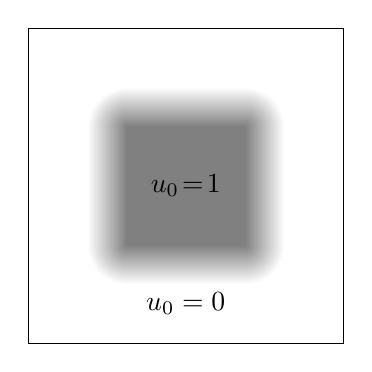
\begin{tikzpicture}[scale=.25]
      \draw (0,0) rectangle (16,16);
      \shade[shading=radial] ( 3, 3) rectangle ( 7, 7);
      \shade[shading=radial] ( 9, 3) rectangle (13, 7);
      \shade[shading=radial] ( 9, 9) rectangle (13,13);
      \shade[shading=radial] ( 3, 9) rectangle ( 7,13);
      \shade[shading angle=0]   ( 5, 3) rectangle (11, 5);
      \shade[shading angle=90]  (11, 5) rectangle (13,11);
      \shade[shading angle=180] ( 5,11) rectangle (11,13);
      \shade[shading angle=270] ( 3, 5) rectangle ( 5,11);
      \filldraw[gray] (5,5) rectangle (11,11);
      \node at (8,8) {$u_0\!=\!1$};
      \node at (8,2) {$u_0=0$};
    \end{tikzpicture}
    \caption{Initial conditions}
  \end{wrapfigure}
  Consider the initial and boundary conditions
  (\ref{ch1:first})--(\ref{ch1:last}) modified as follows:
  \begin{align}
    \label{ch2:first}
    \Gamma_D&=\emptyset \\
    g(x, t) &= \prod_{i=0}^{d-1}\min\{1,\max\{0,\tilde{f}(x_i)\}\} \\
        & \qquad\qquad \tilde{f}(\xi):=0.5-8(|\xi-0.5|-0.25) \nonumber \\
    \label{ch2:last}
    j(x,t)&=0 .
  \end{align}
  The initial condition given by $g$ models a block of constant 1
  concentration in the middle, constant 0 concentration at the border
  and some linear decrease in between.

  On a $16\times16$ or finer grid the initial values can be represented
  exactly by $\mathcal{Q}_1$ and $\mathcal{Q}_2$ finite elements.
  The exact solution will instantly
  become smooth and tend toward the mean over time.  A computed solution is
  only an approximation, and may show different behavior.  Most often it may
  take a long time for the solution to become smooth and, depending on
  the time stepping scheme used, there are spikes oscillating from one
  time step to the next.

  Please implement the initial and boundary conditions
  (\ref{ch2:first})--(\ref{ch2:last}). When implementing $g_\text{ext}$
  you may be tempted to use the function \lstinline!abs()!. This is
  wrong, \lstinline!abs()! is a function from the C-library to compute
  absolute values for \emph{integers}. If a floating point value is
  plugged in, it is truncated to an integer. The correct way is to use
  \lstinline!std::abs()! instead.

  Compile and run your program.
  Remember that the grid needs $16\times16$ elements for the
  $\mathcal{Q}_1$/$\mathcal{Q}_2$ elements to resolve the initial
  condition exactly.  What happens to the interpolated initial condition
  if you use a coarser mesh?

  \paragraph{Step 4: Investigate Maximum Principle}

  \lstset{language=bash} With these preparations done, it is now time to
  actually check how the different discretizations perform.  Run your program
  to produce some output that you can examine in ParaView. Change the
  settings in the ini-file to a $64\times 64$ grid and the time step size
  \lstinline!<dt>!$\,=1/64=0.015625$. Run the simulation until
  \lstinline!<tend>!$\,=4 \cdot\textup{dt}$.
  When examining the solution in ParaView, apply the ``Warp by Scalar''
  filter to get an image distorted into the third dimension according to
  the values of the solution.

  After one time step, the solution computed by $\mathcal{Q}_1$ finite
  elements with Implicit Euler time stepping should be completely
  smooth. The same goes for $\mathcal{Q}_2$ with Implicit Euler.

  With both Crank-Nicolson and Fractional Step $\theta$, both with
  $\mathcal{Q}_1$ and $\mathcal{Q}_2$ the solution should be quite
  non-smooth, i.e.\ there should be some edges visible.  The Fractional
  Step $\theta$ scheme should be smoother than Crank-Nicolson.

  Try to run the simulation with smaller time steps.  How small do you need to
  make the time steps to get smooth solutions with Fractional Step $\theta$?

  Can you get the Crank-Nicolson scheme to produce smooth solutions as well?
\end{Exercise}

\begin{Exercise}{Time Dependent $g$ and $j$}
  Consider now the initial and boundary conditions
  (\ref{ch1:first})--(\ref{ch1:last}) time dependent:
  \begin{align}
    \label{ch3:first}
    \Gamma_D &= \{ x\in\partial\Omega \mid x_0 = 0 \} \\
    g(x,t) &= t/10 \\
    \label{ch3:last}
    j(x,t) &= -(0.5 + \cos(t)/2) .
  \end{align}
  Incorporating the time dependence into the functions $g$ and $j$ is
  easy even if they don't have the time variable as an argument. The
  problem parameter class possesses the member variable \lstinline!t!
  and the member function
  \begin{lstlisting}
    void setTime (Number t_)
    {
      t = t_;
    }
  \end{lstlisting}
  by means of which the correct time is always available. Please
  implement the conditions (\ref{ch3:first})--(\ref{ch3:last}), compile
  and rerun the program. You might also want to increase the final time
  of the simulation. Examine the results in ParaView with the ``Warp by
  Scalar'' filter.
  \paragraph{A short note on time dependent $\Gamma_D$ and $\Gamma_N$:}
  In principle it is possible to implement time dependent $\Gamma_D$ and
  $\Gamma_N$ the same way as for $g$ and $j$. But for conforming spatial
  discretizations there is an important limiting assumption, namely that
  the type of boundary conditions do not change over a time step.
\end{Exercise}

\end{document}

%%% Local Variables:
%%% mode: latex
%%% TeX-master: t
%%% mode: flyspell
%%% ispell-local-dictionary: "american"
%%% End:
